%! TEX root = ./master.tex

\lecture{13}{Week 7}{Linking}
When a project in split into multiple files \code{.c}, they are compiled independently into object files \code{.o}. The linker is then responsible for combining all object files into the final executable. The Unix linker is called \code{ld} but since gcc is actually a wrapper of many programs, it does also the linking part.

When we compile a file using ggc, the \code{-g} flag makes sure that debugging information remains in the executable.

\subsubsection{Why Linkers}
\begin{description}
    \item[Modularity:] Linkers allow to break a project into many small pieces on which one can work independently. Furthermore, linkers allow to build libraries.
    \item[Efficientcy:] Linkers allow to write efficient code in two ways:
        \begin{itemize}
            \item Compiling takes time. Then only one file changes, it would be wasteful to recompile also the unchanged files. 
            \item We can put function which may be reused in a dedicated file. This allow for simple reuse as well as lower memory usage when loading this function, since the file only contains code we actually need.
        \end{itemize}
\end{description}
\paragraph{Modularity}

\subsubsection{What does a Linker do?}
Linking is a two-step process:
\begin{description}
    \item[1. Symbol Resolution:] Programs define and reference symbols. Symbols are function names and variables. The symbols definitions get stored into the symbol table by the compiler. This is an array of stucts where each entry includes symbol name, type, size and location. The linker then associates each symbol reference with exactly one symbol definition.
    \item[2. Reallocation:] The linker merges separate code and data section into a single section. This requires the reallocation of the symbols from their relative location in the \code{.o} files to their final absolute memory location in the executable.
\end{description}

\subsubsection{Object Files}
There exist three different kinds of object files (modules):
\paragraph{Relocatable Object Files}
They have the extension \code{.o} and each single file is the product of a compiled source file. They contain code and data which is in a format, such that it can be combined with other relocatable object files to form an executable. 

\paragraph{Executable Object Files}
They contain code and data which can be directly copied to memory and executed.

\paragraph{Shared Object File}
They have the \code{.so} extension. These are special object files which have the property, that they can be loaded and linked dynamically at runtime, into memory.

\paragraph{Executable and Linkable Format (ELF)}
All mentioned object files types share the same format. The ELF is the standard finery format for object files and the generic name for such object files is ELF binary.

A section referees to bits of a file where segments referees to bits in memory.

The general format is as follows:
\begin{description}
    \item[Elf Header:] Tells that this file is in the ELF format as well as provides information about endianess, word size, machine type, file type etc.
    \item[Segment Header Table:] Contains information about the page size, virtual address memory segments (where is stack, heap etc), segment size.
    \item[.text section:] Machine code given by the compiler.
    \item[.rodata section:] Read-only data like the jump-table.
    \item[.data section:] Initialized global variables. The last segment tells where the .bss section starts.
    \item[.bss section:] Uninitialized global variables. Since they have no value, it is normally smaller than the data segment. Called \textit{Block Started by Symbol} or \textit{Better Save Space}.
    \item[.symtab section:] Symbol table and the names of procedures and static variables.
    \item[.rel.text section:] Reallocation information for .text section (addresses of instruction which need to be modified as well as instruction for modifying).
    \item[.rel.data section:] Reallocation information for .data section (addresses of pointer data which need to be modified).
    \item[.debug section:] Information fo symbolic debugging with \code{gcc -g}.
    \item[Section Header Table:] Offset and sized of each section.
\end{description}

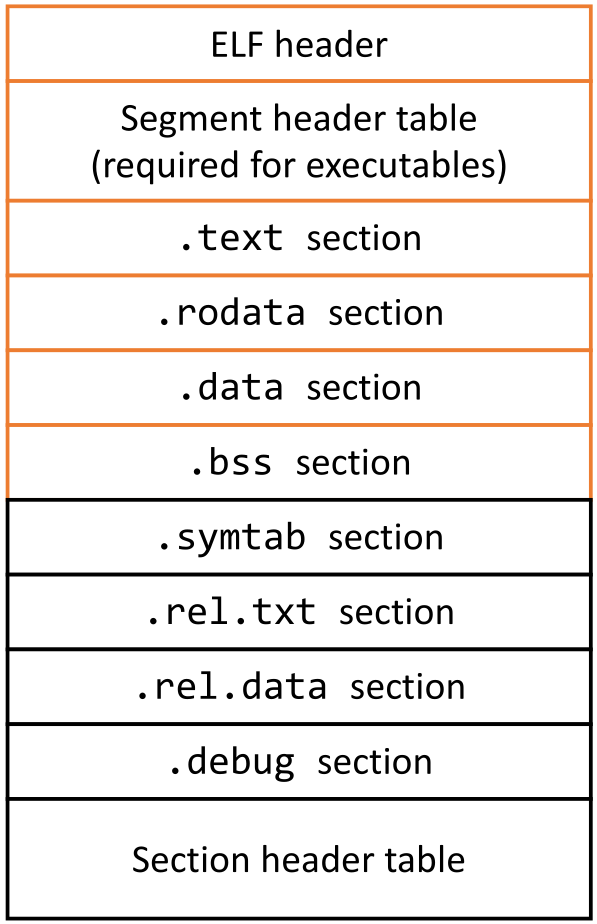
\includegraphics[width=0.8\textwidth]{13_elfformat.png}

\subsubsection{Linker Symbols}
There are three types of symbols:
\paragraph{Global Symbols}
Symbols which are defined as globals in a certain module.

\paragraph{External Symbols}
Symbols which are referenced in a certain module, but defined in another module. One can prepend external symbols by \code{extern}. This is not required, nevertheless, one should always do it for good practice.

\paragraph{Local Symbols}
Symbols which are defined and referenced only in a certain module. However, they are \textbf{not} local program variables. Linkers are not aware of any local program variables.

\paragraph{Example Linker}
Given the following code, we can find the symbols and their type:

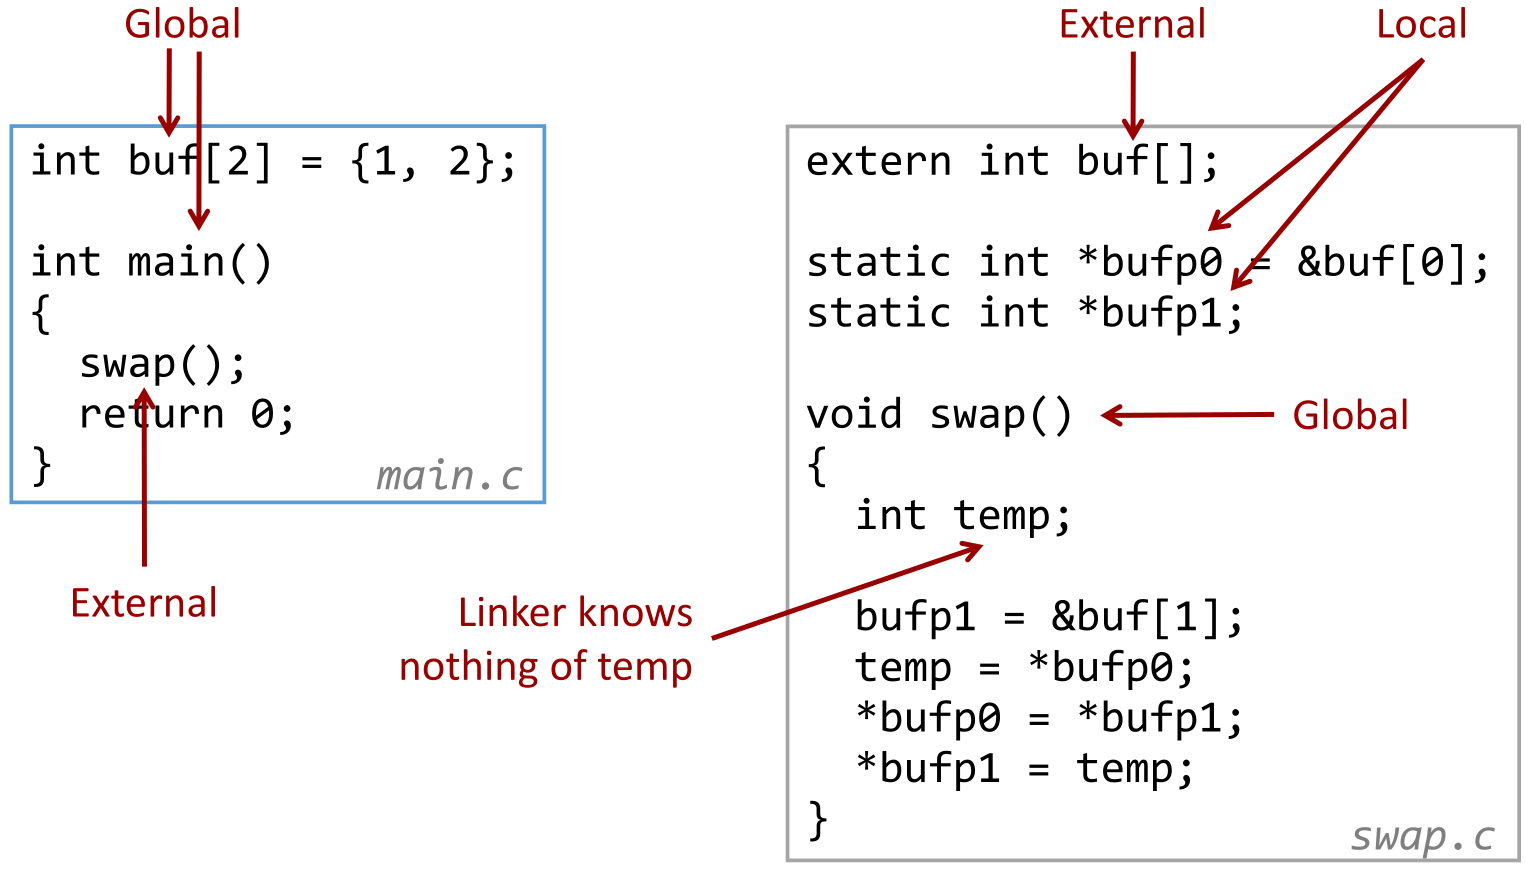
\includegraphics[width=0.8\textwidth]{13_linkersymbols.png}

The linker combines them as follows into an executable. The system code and data is stuff the compiler sees but we do not.

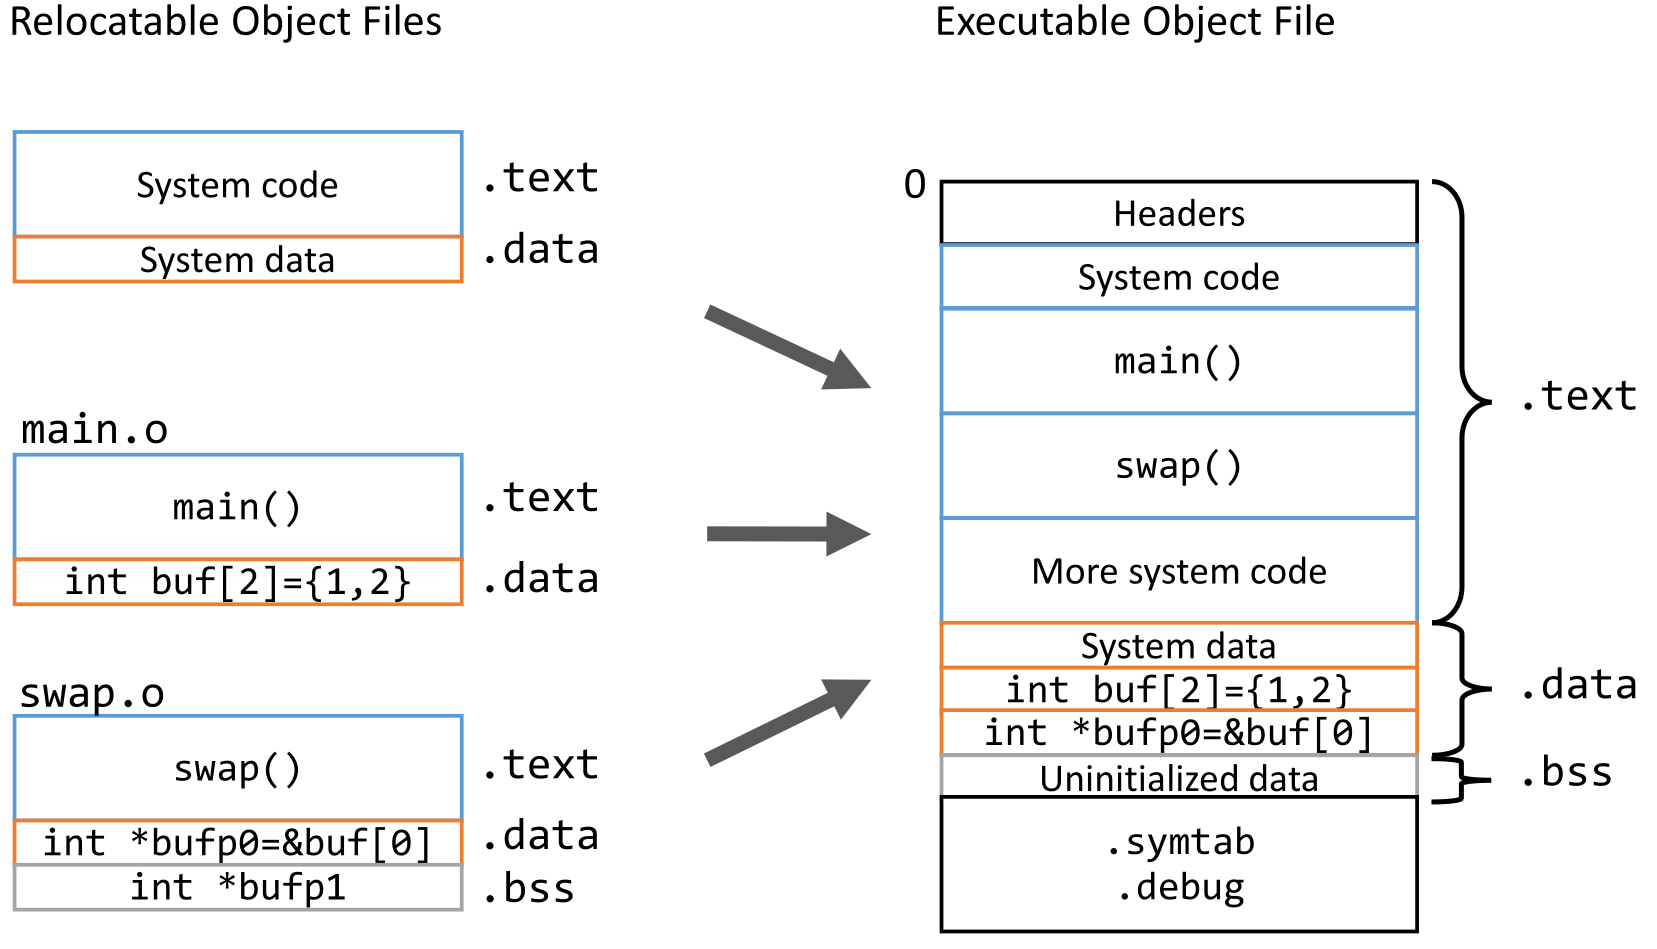
\includegraphics[width=0.8\textwidth]{13_realocatingCodeData.png}

In the disassembled .tex section of main.o we see, that the compiler does not know where swap is. Instead, it inserted an entry into the symbol table (the string in read). String tells that at address $a$ there are $4$ bytes which need to be filled with the address of the function called \code{swap}. The \code{R\_X86\_64\_PC32} means it is a reallocation entry for a x86-32 processor which used pc relative $32$ addressing. This information allows the linker to fill in the right address.

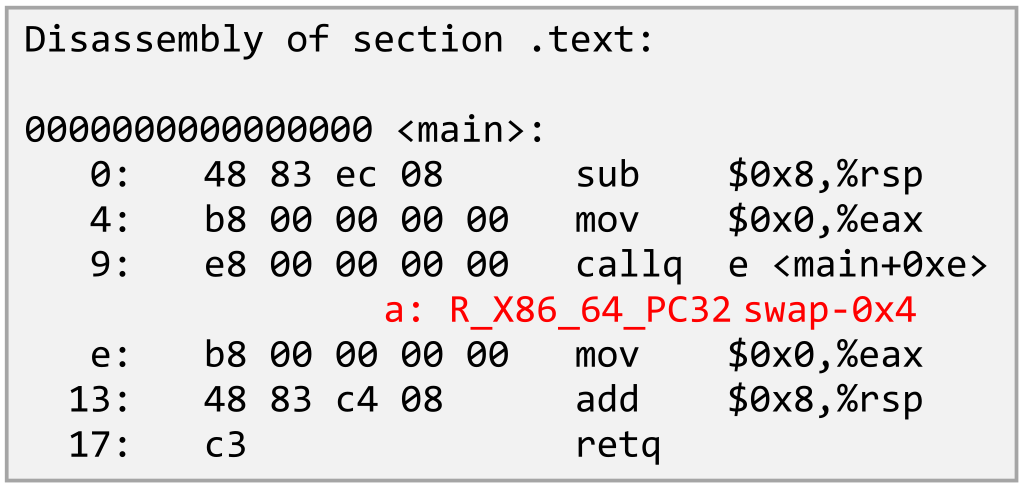
\includegraphics[width=0.8\textwidth]{13_ex_maintext.png}

The disassembled .data section we can see the global two integer.

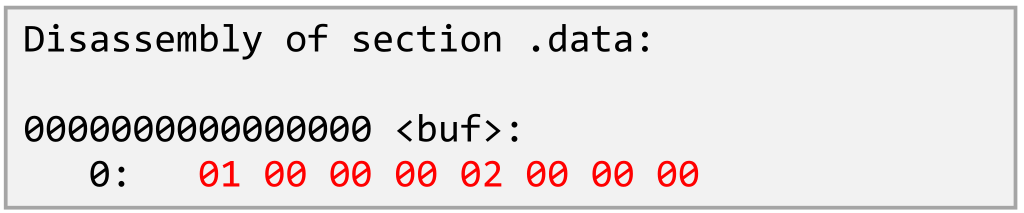
\includegraphics[width=0.8\textwidth]{13_ex_maindata.png}

The first movq instruction has again two $4$ byte long addresses of zero. The first address is again a PC relative $32$ offset reallocation instruction. It is the unallocated \code{bufp1} symbol and hence, it is referred to as \code{.bss-0x8}. The second address is again a reallocation entry but it is a $32$ bit scalar value, which is referred too as \code{buf+0x4}.

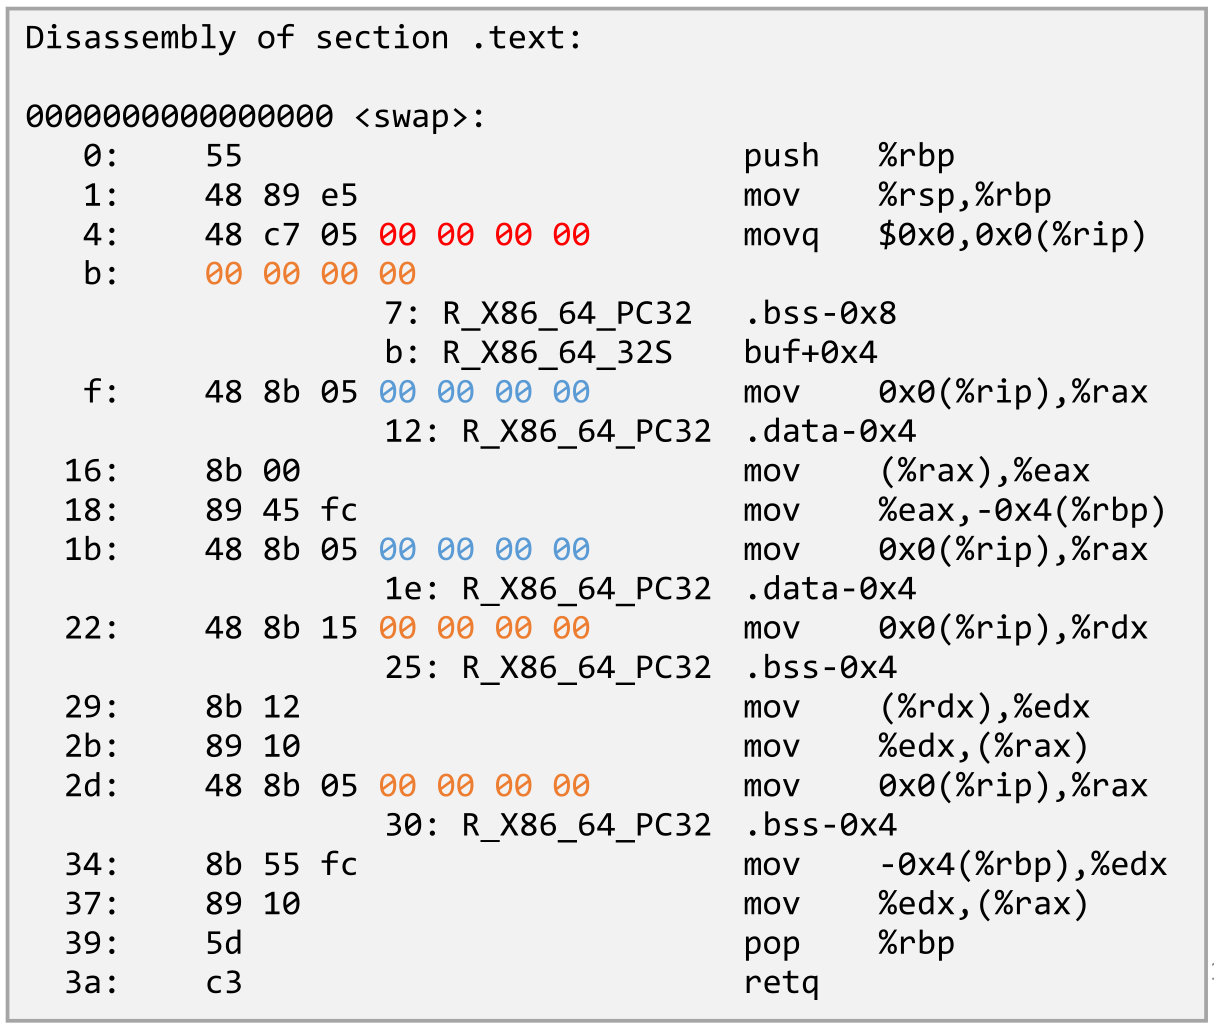
\includegraphics[width=0.8\textwidth]{13_ex_swaptext.png}

In the data section we find the \code{buf}. In the bss section we find the \code{bufp1} symbol. it has $8$ bytes, but they are actually not in the file, it is just recorded that they should be there.

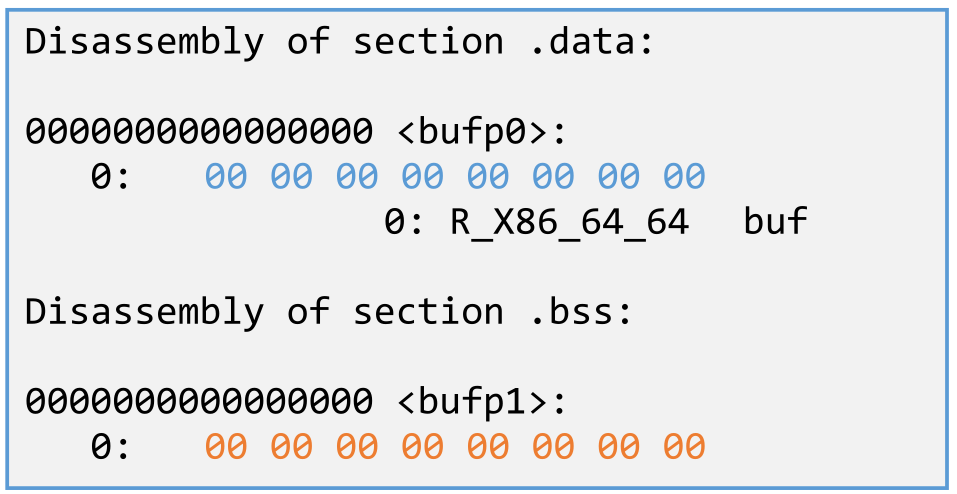
\includegraphics[width=0.8\textwidth]{13_ex_swapdatabss.png}

The linker takes the previously discussed files, and puts them into a single executable. The .text section looks as follows. The file looks very familiar, but the missing addresses were filled in (the linker reallocated the addresses). 

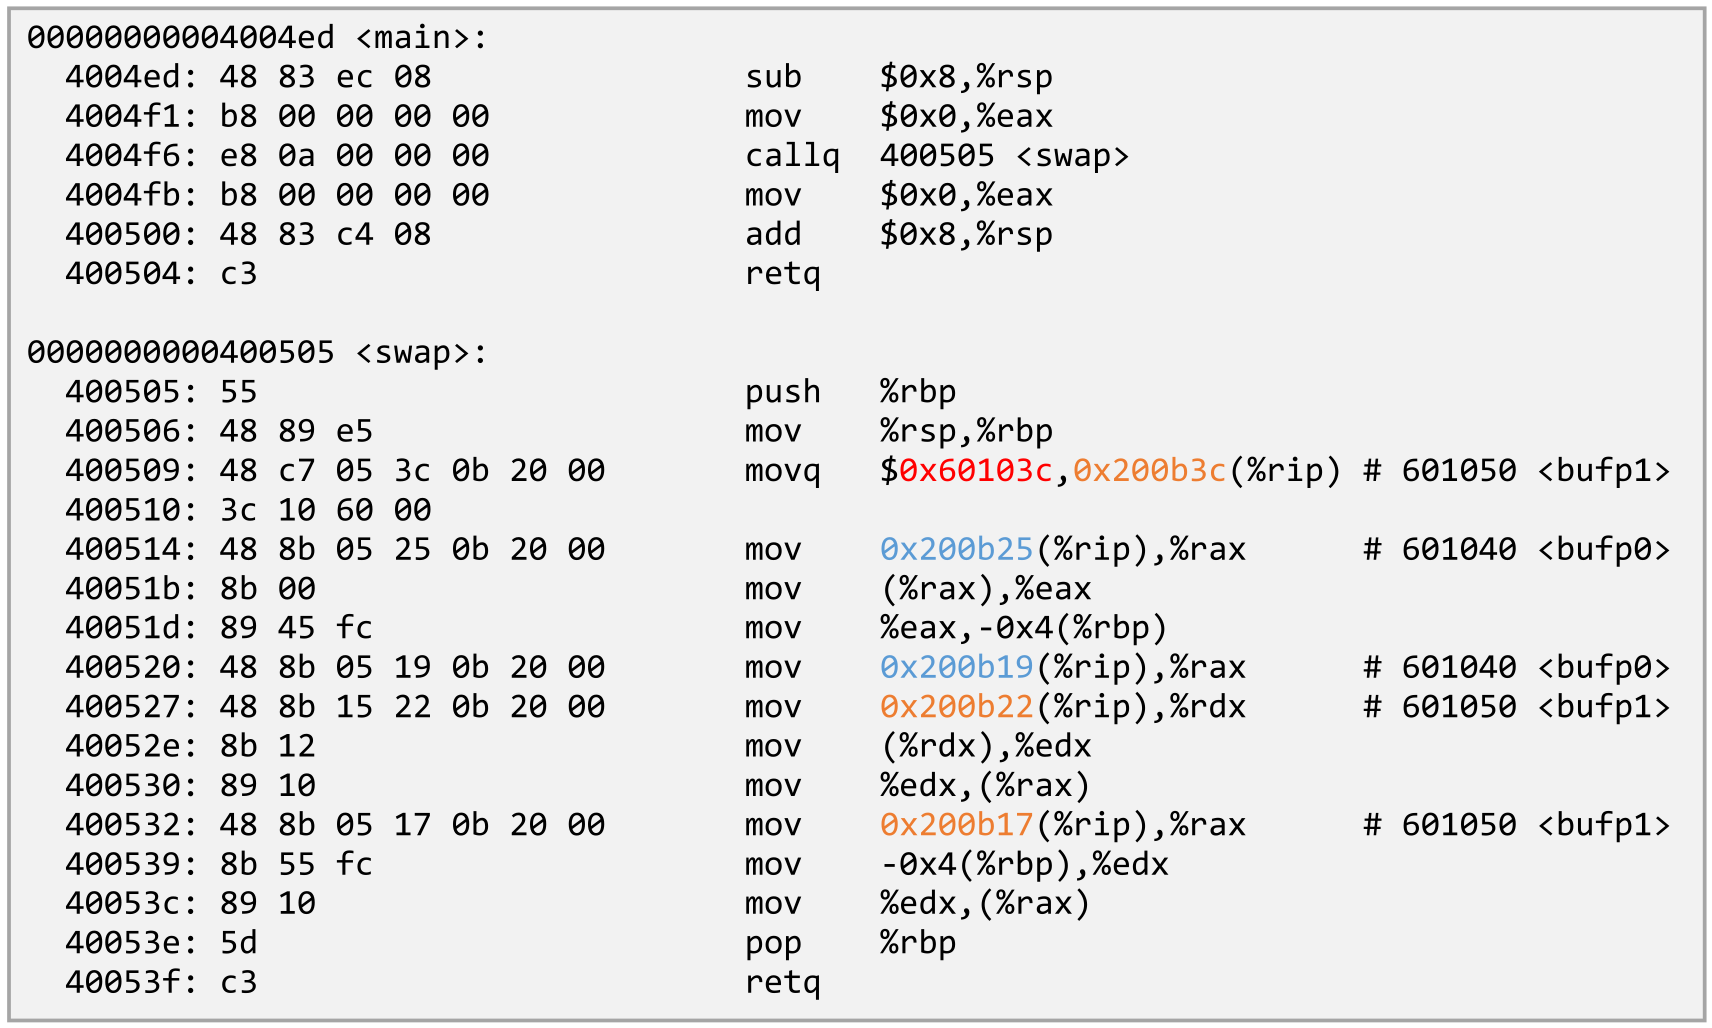
\includegraphics[width=0.8\textwidth]{13_ex_exectext.png}

And the .data and .bss. We notice that all addresses are only $8$ bytes long. The reason is in order to save space. The compiler uses relative addresses and the linker figures out what this address is.

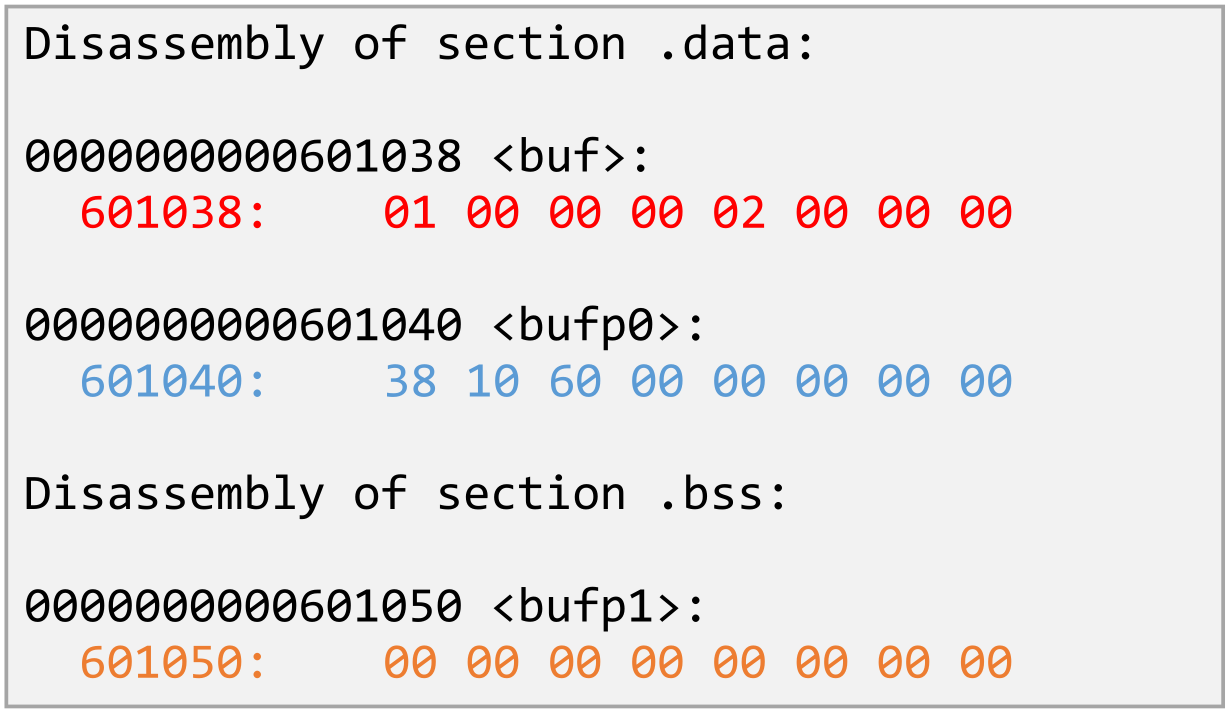
\includegraphics[width=0.8\textwidth]{13_ex_exec_databss.png}

\paragraph{Strong and Weak Symbols}
\begin{description}
    \item[Strong:] Procedures and initialized globals
    \item[Weak:] Uninitialized globals
\end{description}

\paragraph{Linker's Symbol Rules}
Then multiple symbols with the same name are given the linker proceeds as follows:

\begin{enumerate}
    \item Multiple string symbols are not allowed. This leads to a linker error.
    \item When given a strong and multiple weak symbols, the liner always chooses string symbol. So, references to the weak symbol resolve to the strong one.
    \item When given multiple weak symbols, the linker picks one arbitrary. This can lead to weird problems. E.g. when there are two structs with the same name and same size, but different fields (one has two ints, the other one double), the linker may select one at random and when writing to e.g. the address of the first int, we may be dealing with a double of the size of both ints. This problem may also arise when we combine code which was compiled by different compiler which have different alignment rules.
\end{enumerate}

\paragraph{Some Puzzles}
Some Linking Puzzles:

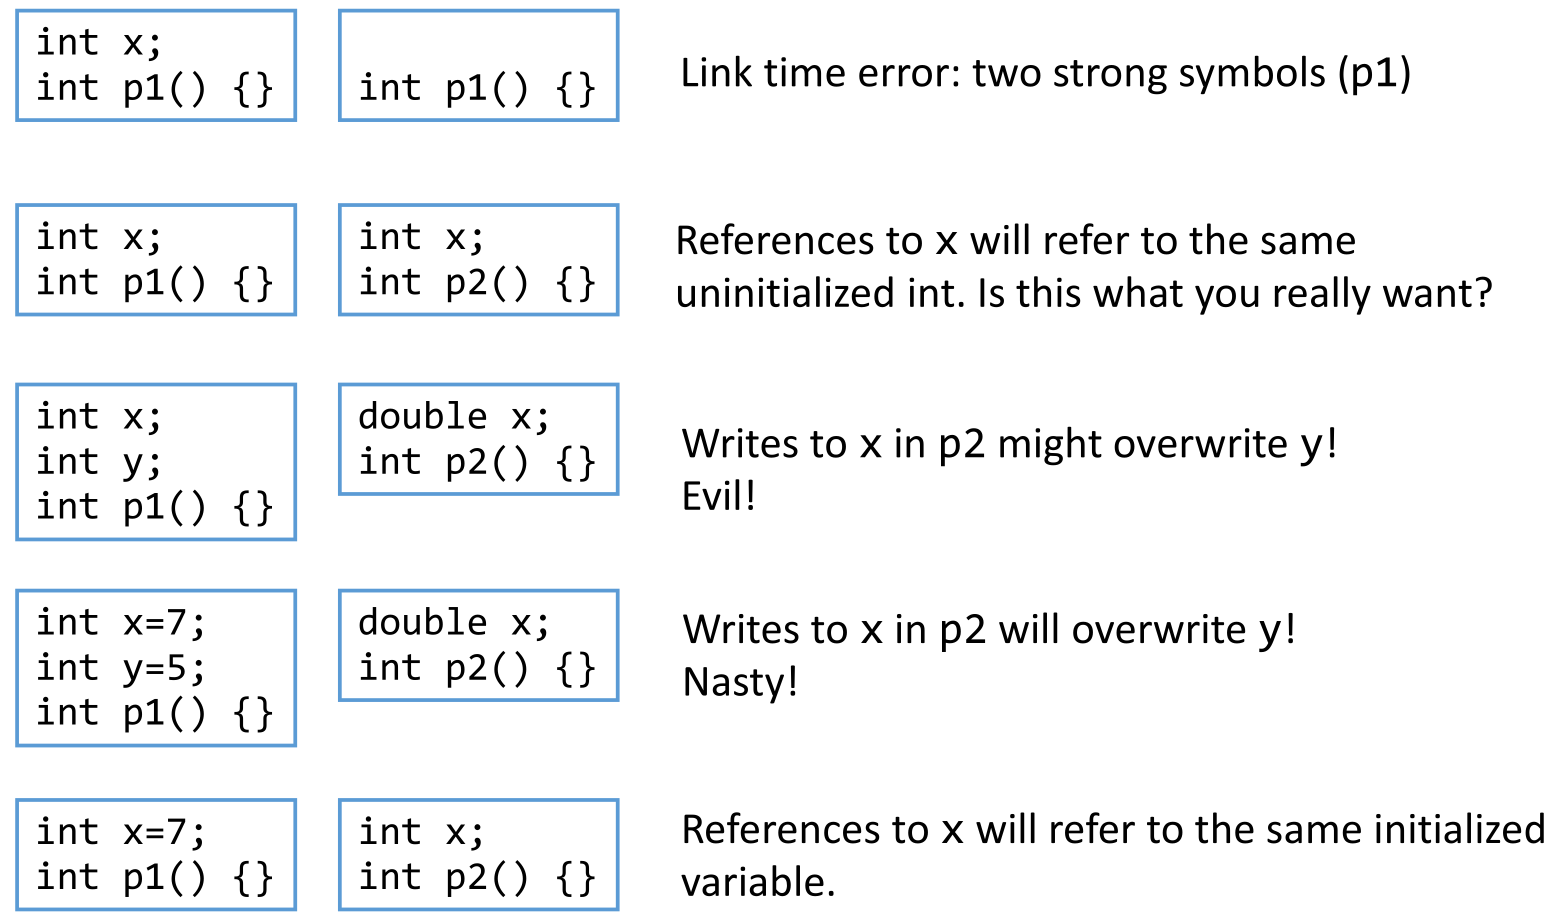
\includegraphics[width=0.8\textwidth]{13_linkerpuzzles.png}

\paragraph{Global Variables}
Globals can cause many issues. Besides the already disused ones, it may also quickly happen that different programs declare globals with the same name. Good practice is to avoid them when possible. If not, one should at least initialized them. An when using an external global, one should always prepend it by \code{extern}.

\subsubsection{Static Libraries}
We may want to package commonly used functions into a library. Trivial ways to accomplish that is by putting all function into a single source file or by putting each function into a separate file. Both methods have some downsides. While the first methods is very space and time inefficient, the second methods puts a burden on the programmer to link the appropriate binaries into their programs.

Static libraries solve this problem. They have the extension \code{.a} and the concatenate related relocatable object files into a single archive file. The linker tries to resolve unresolved external references by looking for that symbol in one or multiple archived. On success, the linker links the object file into the executable.

The following diagram shows the usage of static libraries:

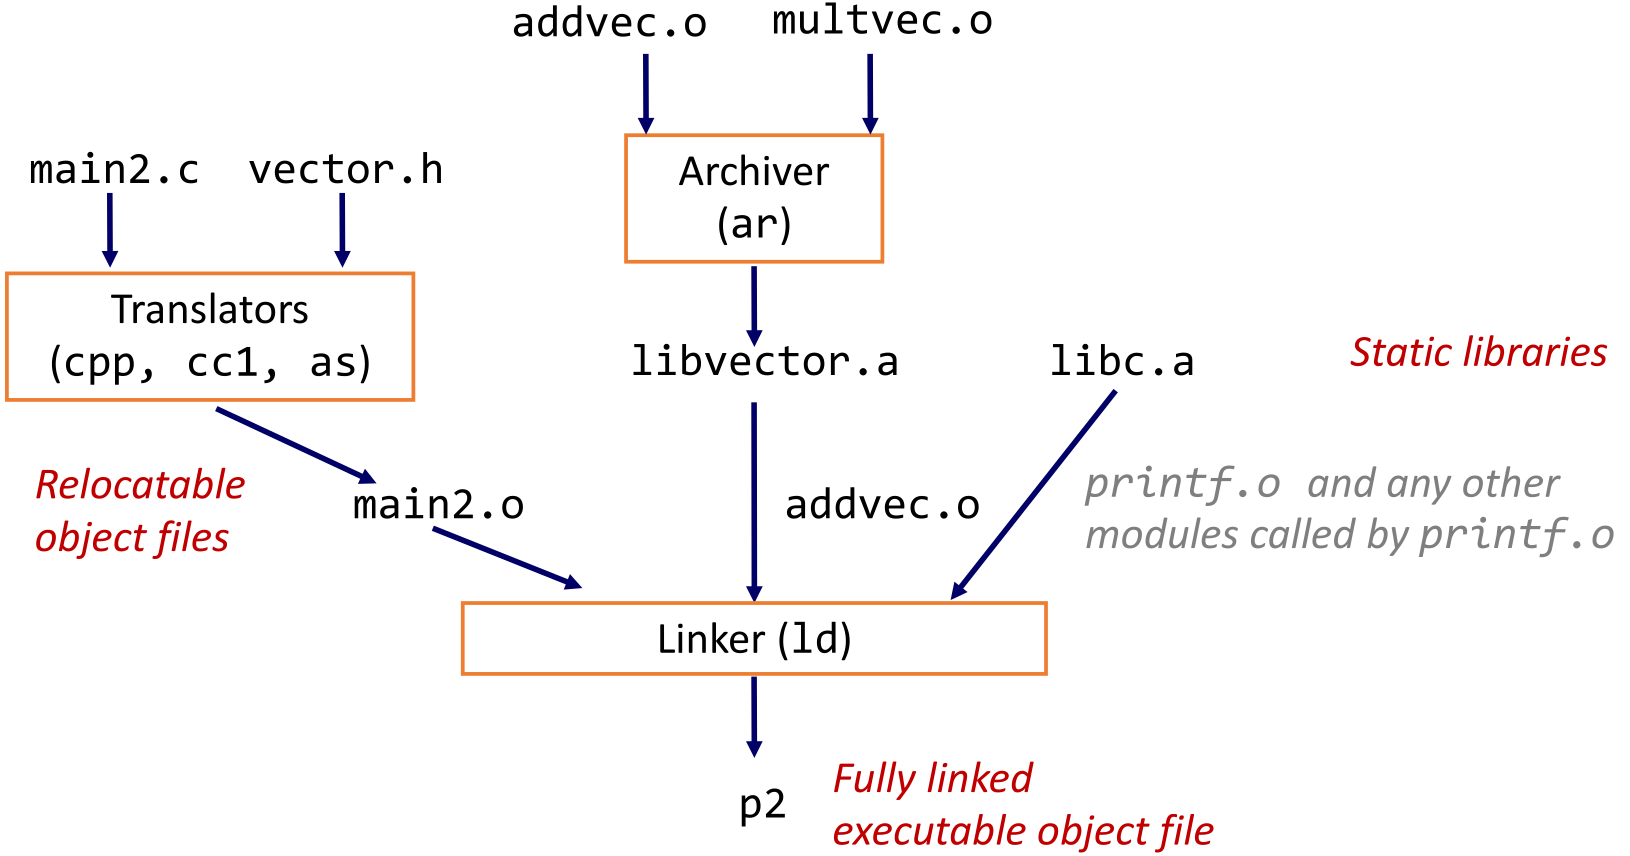
\includegraphics[width=0.8\textwidth]{13_staticlibrarydiagram.png}

\paragraph{Build Archives}
The archiver \code{ar} is used to create such archives:

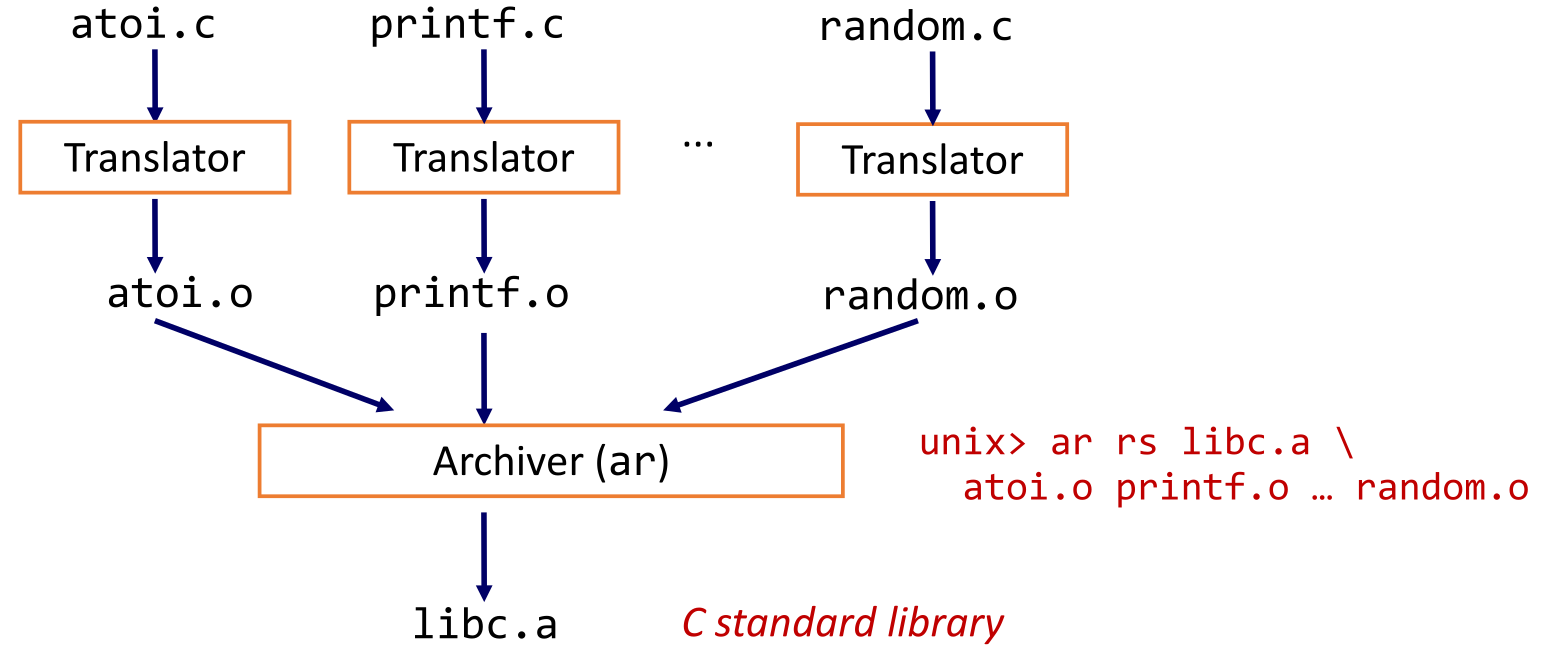
\includegraphics[width=1\textwidth]{13_staticlibrary.png}

The archiver allows incremental updates. This means that when a function changes, only the source of that file is recompilation and the .o file is replaced in the archive.

How does the linker know where these archives are? There are certain defaults directories. To include certain libraries, it is also possible to load it with \code{gcc -lm} where \code{m} is the name of the library (in this case libm (the math library)).

\paragraph{How Linker Resolve External References}
The linker scans the .o files and .a archives in the ordre they were provided to the command. During the scan, it weeks a list of currently unresolved reference. Always when a new archive .a or object .o file is encountered, it tries resolve unresolved reference and updates the unresolved references list. If at the end of this process there are unresolved reference, this leads to an error.

The main problem is, that the linker does only one pass of this algorithm. Since files are scanned in the order they are provided, one should put libraries at the end of the command. E.g. \code{gcc -L. libtest.o -lmine} instead of \code{gcc -L. -lmine libtest.o}.

\paragraph{Loading an Executable Object File}
When loading an executable, different sections are put into corresponding segments in memory. It used to be the way, the executables would be put directly into memory in reversed order.

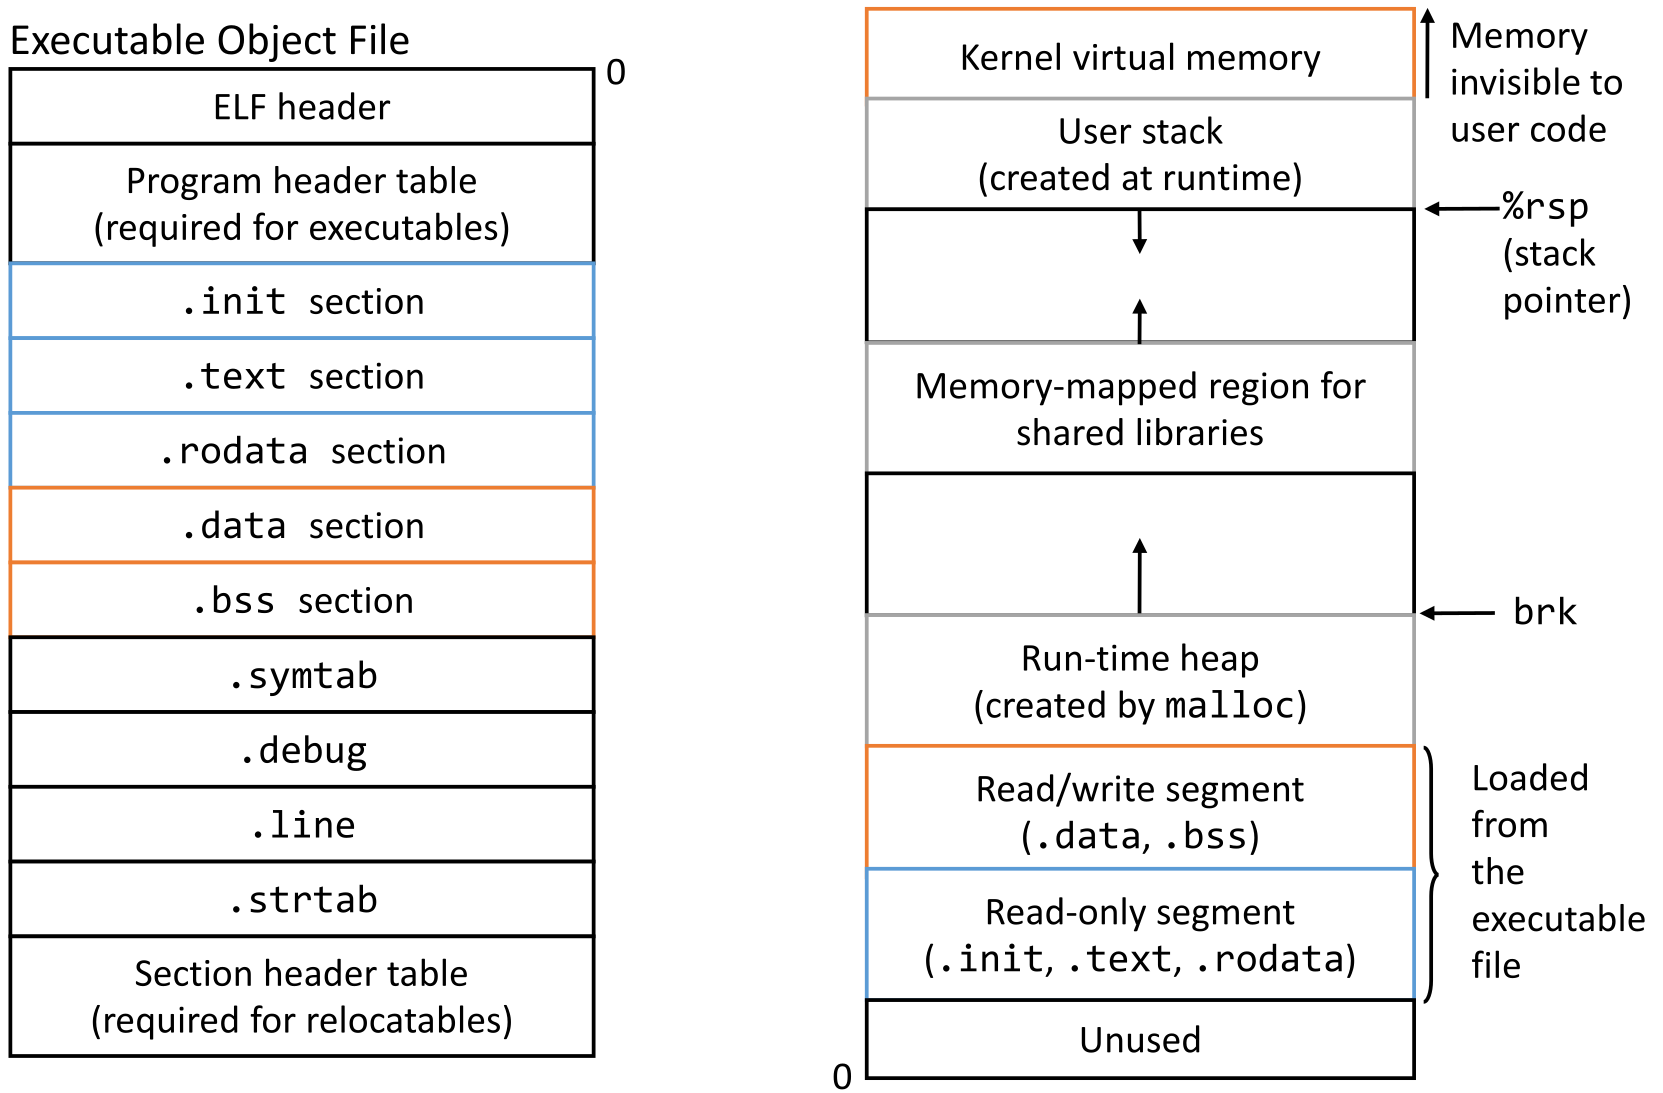
\includegraphics[width=0.8\textwidth]{13_loadingexecutables.png}

\subsubsection{Shared Libraries}
Since when using static libraries, all code is copied into the executable, one has to recompile the program, when the library is updated. Further, the code is always duplicated. Therefore, static libraries are only actually used during the building process and shared libraries in production.

Shared libraries provide object files containing code and data which get linked into a program dynamically during load-time or run-time.

Shared libraries are also called dynamic link libraries (DLLs) and they can be shared between multiple processes.

\paragraph{Load-Time Linking} is automatically handled by the dynamic linker \code{ld-linux.so}. The following graphic depicts the procedure:

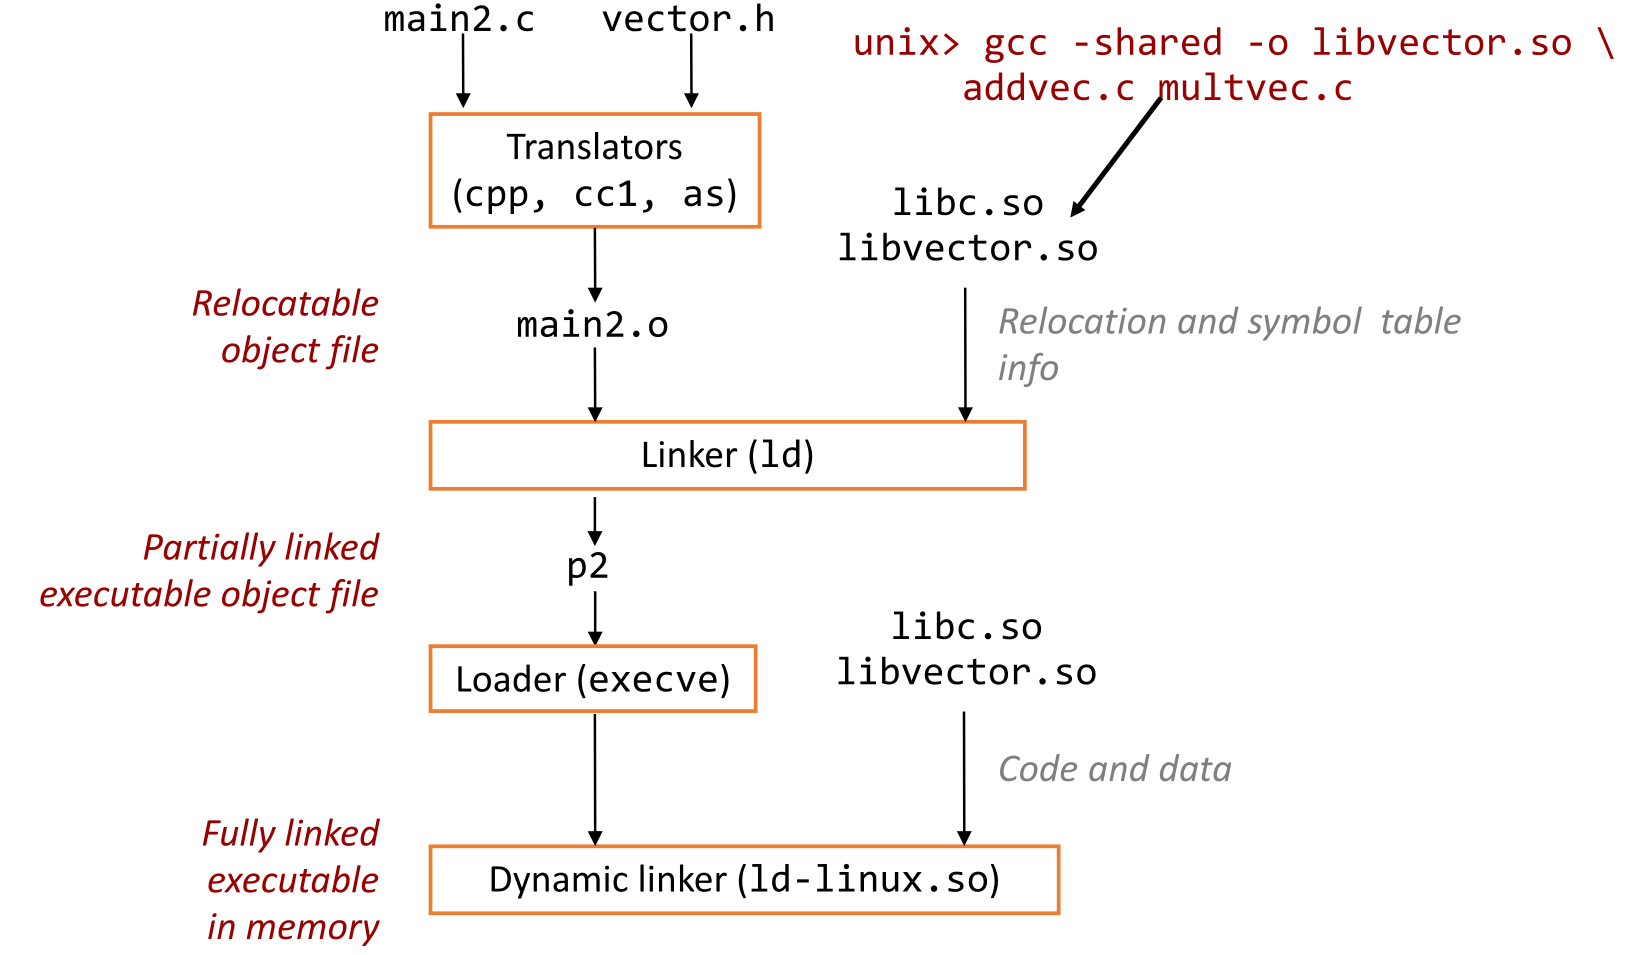
\includegraphics[width=0.8\textwidth]{13_dynamicLinking.png}

\paragraph{Run-Time Linking} is done by calls to \code{dlopen()} interface.

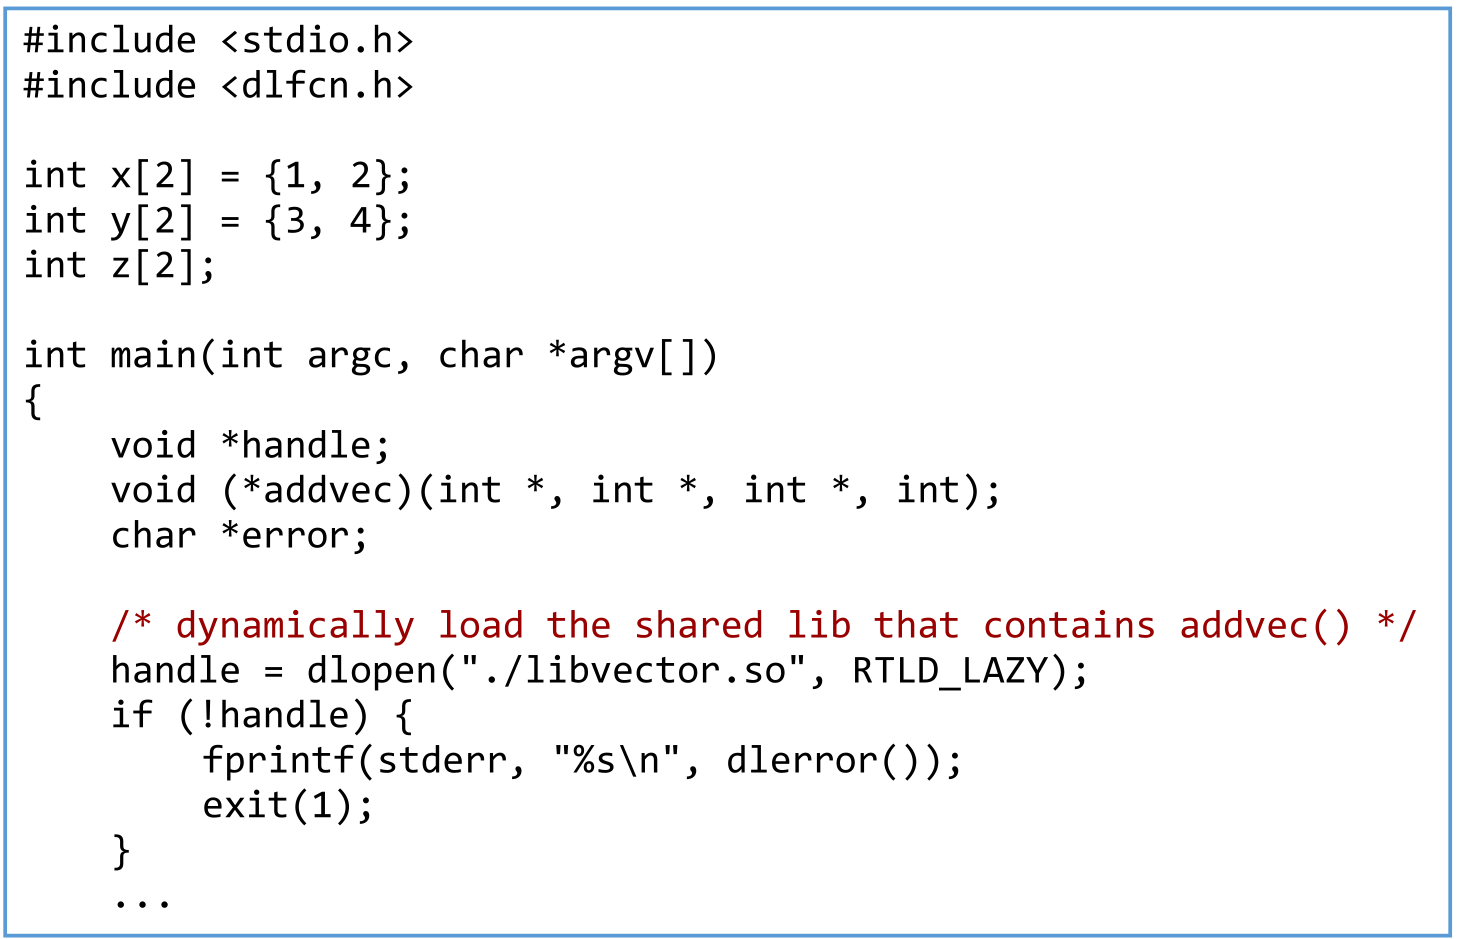
\includegraphics[width=0.8\textwidth]{13_runtimeI.png}

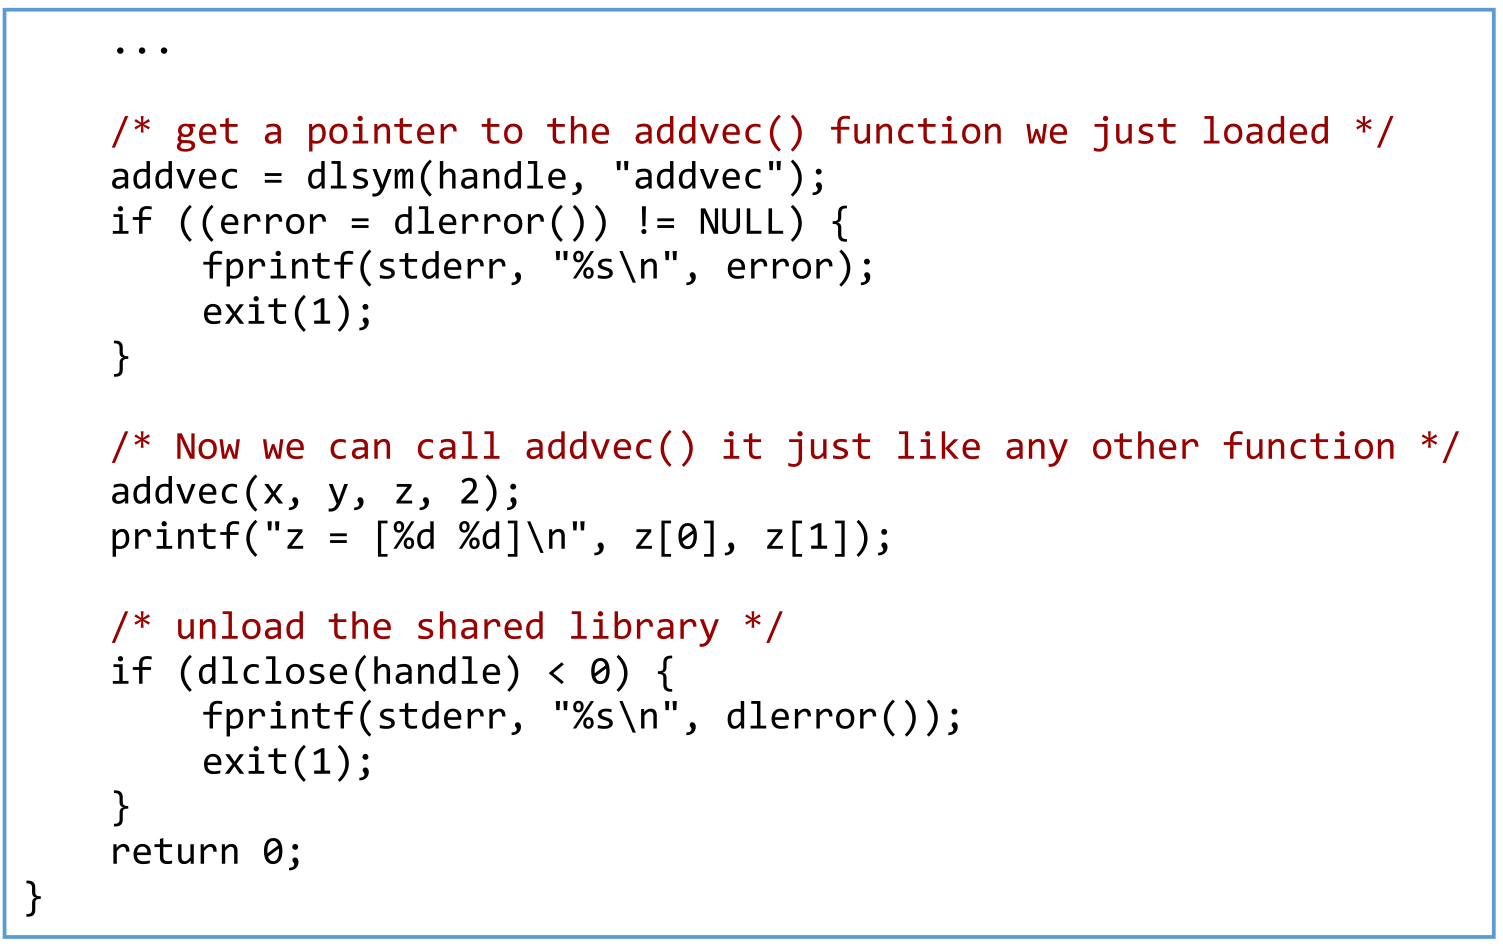
\includegraphics[width=0.8\textwidth]{13_runtimeII.png}





main+addr is used then the location of the function is unknown. The linker is responsible to fill in the missing address at address $a$. The red string is stored in the symbol table. 

.bss-0x8 stands for the rip we do not know. The buf+0x4 is a scalar value and is the 

compiling p2 alone, we get something in the .bss called foo
compiling p1 alone, we get something in the .data called foo

if the two files are linked together, we only get one foo, and this is the p1 because the linkers sees assumes that the foos are equivalent
